\lab{GMRES}{GMRES}
\objective{The Generalized Minimal Residuals (GMRES) algorithm is an iterative Krylov subspace method for efficiently solving large linear systems.
In this lab we implement the basic GMRES algorithm, then make an improvement by using restarts.
We then discuss the convergence of the algorithm and its relationship with the eigenvalues of a linear system.
Finally, we introduce SciPy's version of GMRES.}


\begin{comment}
\section*{The Arnoldi Iteration and Approximate Solutions} % ==================

Let $A$ be an $m\times m$ matrix (real or complex), where $m$ is very large,
and let $b \in \mathbb{F}^m$ ($\mathbb{F}$ may either be the real or complex numbers).
Let $\mathcal{K}_n$ denote the order-$n$ Krylov subspace generated by $A$ and $b$.
In each iteration, we consider the least squares problem
\begin{equation}
\underset{x \in \mathcal{K}_n}{\text{minimize}}\qquad \|b-Ax\|_2.
\label{eq:GMRES_lstsq1}
\end{equation}
Now if $x \in K_n$, then $x$ can be expressed as a linear combination of basis vectors $b, Ab, \ldots, A^{n-1}b$, i.e.
\[
x = y_1b + y_2Ab + \cdots + y_nA^{n-1}b.
\]
If we let $K_n$ be the matrix whose columns are $b, Ab, A^{2}b, \cdots, A^{n-1}b$, then we can write this simply as
$x = K_n y$.
Then the solution of the least squares problem is the vector $K_{n}y$ such that $\|b-A K_{n}y\|_2$ is minimized.
\begin{figure}
\includegraphics[width=\textwidth]{figures/LeastSquares.pdf}
\caption{GMRES involves solving the least squares problem repeatedly.}
\end{figure}

The major drawback of this approach is that it relies on the matrix $K_n$, which tends to be ill-conditioned due to its columns
being far from orthogonal (as discussed in Lab \ref{lab:kry_arnoldi}).
%To see this, suppose there is an eigenbasis for $A$ with associated eigenvalues, and suppose $\lambda$ is the largest eigenvalue.
%Then $\lambda^n$ is an eigenvalue of $A^n$.
%Since $\lambda$ is bigger than the other eigenvalues of $A$, $\lambda^n$ may be much, much bigger than the other eigenvalues of $A^n$,
%which are simply the eigenvalues of $A$ raised to the $n$th power.
%Thus the eigenvector associated with $\lambda$ often begins to dominate as we progress, with the end result being that the columns of
%$K_n$ become nearly linearly dependent.
The easiest fix in this situation is to use the Arnoldi iteration so that we have an orthonormal basis for $\mathcal{K}_n$ to work with.
Not only does this alleviate the problem of ill-conditioning, it also allows us to optimize in other ways, due to the special
structure of the matrices produced.

Let $q_1,\ldots, q_n$ be the orthonormal basis for $\mathcal{K}_n$ obtained by the Arnoldi iteration, and let $Q_n$ be the matrix
having these vectors as its columns.
Recall that $q_1 = b/\|b\|_2$.
Finally, let $H_n$ be the $(n+1)\times n$ upper Hessenberg matrix generated by the Arnoldi iteration, and let $e_1=(1,0,\cdots,0)$.

In this orthonormal basis, $x \in \mathcal{K}_n$ implies that there is some vector $y$ such that $x = Q_n y$.
Further, it is not hard to check that the matrices generated by the Arnoldi iteration satisfy the equation
\[
AQ_n = Q_{n+1}H_n.
\]
We also have the identity
\[
b = \|b\|_2q_1 = \|b\|_2Q_{n+1}e_1.
\]
Putting all of this together, we can rewrite the objective function of our least squares problem as follows:
\begin{align*}
\|b - Ax\|_2 &= \|Ax - b\|_2\\
&= \|AQ_ny - b\|_2\\
&= \|Q_{n+1}H_ny - \left(\|b\|_2Q_{n+1}e_1\right)\|_2\\
&= \|Q_{n+1}\left(H_n y - \|b\|_2e_1\right)\|_2.
\end{align*}

The matrix $Q_{n+1}$ has orthonormal columns, but it does not have enough columns to be a unitary matrix.
Let us extend the set $q_1,\ldots, q_{n+1}$ to an orthonormal basis $q_1,\ldots,q_{n+1},q_{n+2},\ldots,q_m$
of our space, and let $Q'$ be the matrix whose columns are equal to these vectors.
Then $Q'$ is now a unitary matrix, and hence preserves the norm, i.e. $\|Q'z\|_2 = \|z\|_2$ for all $z \in \mathbb{F}^m$.
Given $x \in \mathbb{F}^{n+1}$, if we define $x' \in \mathbb{F}^m$ to be
\[
x' =
\begin{bmatrix}
  x\\
  0\\
  \vdots\\
  0
\end{bmatrix},
\]
then you can easily check that
\[
Q'x' = Q_{n+1}x.
\]
From this, we deduce that
\begin{align*}
\|Q_{n+1}x\|_2 &= \|Q'x'\|_2\\
& = \|x'\|_2\\
&= \|x\|_2.
\end{align*}
Hence, we conclude that
\[
\|Q_{n+1}\left(H_n y - \|b\|_2e_1\right)\|_2 = \|H_n y - \|b\|_2e_1\|_2.
\]
Thus, the least squares problem given by \ref{eq:GMRES_lstsq1} is equivalent to the problem
\begin{equation}
\underset{y \in \mathbb{F}^n}{\text{minimize}}\qquad \|H_n y - \|b\|_2e_1\|_2.
\label{eq:GMRES_lstsq2}
\end{equation}
If $y$ is the solution to this problem, then the solution to \ref{eq:GMRES_lstsq1}, and hence an approximate
solution to $Ax = b$ is given by $x=Q_n y$.

We can measure how good our approximate solution is by considering the residual, which we define to be
\[
\frac{\|Ax-b\|_2}{\|b\|_2}.
\]
We can express this residual in terms of $y$ as follows:
\begin{equation}
\frac{\|H_n y - \|b\|_2e_1\|_2}{\|b\|_2}.
\label{eq:GMRES_residual}
\end{equation}
\end{comment}

\section*{The GMRES Algorithm} % ==============================================

GMRES is an iterative method that uses Krylov subspaces to reduce a high-dimensional problem to a sequence of smaller dimensional problems.
Let $A$ be an invertible $m \times m$ matrix and let $\b$ be a vector of length $m$.
Let $\mathcal{K}_n(A, \b)$ be the order-$n$ Krylov subspace generated by $A$ and $\b$.
Instead of solving the system $A\x = \b$ directly, GMRES uses least squares to find $\x_n \in \mathcal{K}_n$ that minimizes the residual $r_n = \|\b - A\x_n\|_2$.
The algorithm terminates when this residual is smaller than some predetermined value.
In many situations, this happens when $n$ is much smaller than $m$.

The GMRES algorithm uses the Arnoldi iteration for numerical stability.
The Arnoldi iteration produces $H_n$, an $(n+1)\times n$ upper Hessenberg matrix, and $Q_n$, a matrix whose columns make up an orthonormal basis of $\mathcal{K}_n(A, \b)$, such that $AQ_n = Q_{n+1}H_n$.
The GMRES algorithm finds the vector $\x_n$ which minimizes the norm $\norm{\b - A\x_n}_2$, where $\x_n = Q_n \y_n  + \x_0$ for some $\y_n \in \mathbb{R}^n$.
Since the columns of $Q_n$ are orthonormal, the residual can be equivalently computed as
\begin{equation}
\qquad \|\b - A\x_n\|_2 = \|Q_{n+1}(\beta \e_1 - H_n \y_n)\|_2 = \|H_n \y_n - \beta \e_1\|_2.
\label{eq:GMRES_lstsq1}
\end{equation}

Here $\e_1$ is the vector $[1, 0, \ldots, 0]\trp$ of length $n+1$ and $\beta=\norm{\b - A\x_0}_2$, where $\x_0$ is an initial guess of the solution.
% (Ordinarily this guess is zero; however, a modified version of the algorithm will be discussed in a later section, in which nonzero guesses will be used.)
Thus, to minimize $\norm{\b - A\x_n}_2$, the right side of (\ref{eq:GMRES_lstsq1}) can be minimized, and $\x_n $ can be computed as $\x_n=Q_n \y_n + \x_0$.

\begin{comment}
so that instead of solving \eqref{eq:GMRES_lstsq1}, at the $n$th iteration we solve
\begin{equation}
\underset{\y \in \mathbb{F}^n}{\text{minimize}}\qquad \|H_n \y - \|\b\|_2\e_1\|_2.
\label{eq:GMRES_lstsq2}
\end{equation}
Here, $H_n$ is the $(n+1)\times n$ upper Hessenberg matrix generated by the Arnoldi iteration and $\e_1$ is the vector $(1, 0, \ldots, 0)$ of length $n+1$.
If $\y$ is the minimizer for the $n$th iteration of \eqref{eq:GMRES_lstsq2}, then the residual is
\begin{equation}
\frac{\|H_n \y - \|\b\|_2\e_1\|_2}{\|\b\|_2},
\label{eq:GMRES_residual}
\end{equation}
and the corresponding minimizer for (\ref{eq:GMRES_lstsq1}) is $Q_n\y$, where $Q_n$ is the matrix whose columns are $\q_1, \ldots, \q_n$ as defined by the Arnoldi iteration.
This algorithm is outlined in Algorithm \ref{alg:gmres}.
For a complete derivation see [TODO: ref textbook].
\end{comment}

\begin{algorithm}[H]
\begin{algorithmic}[1]
\Procedure{GMRES}{$A$, $\b$, $\x_0$, $k$, \li{tol}}
	\State $Q \gets \allocate{\size{\b}}{k+1}$			\Comment{Initialization.}
	\State $H \gets \zeros{k+1}{ k}$
	\State $r_0 \gets \b - A(\x_0)$
	\State $Q_{:,0} = r_0/\norm{r_0}_2$
    \For{$j=0\ldots k-1$}							\Comment{Perform the Arnoldi iteration.}
        \State $Q_{:,j+1} \gets A(Q_{:,j})$
        \For{$i=0\ldots j$}
            \State $H_{i,j} \gets Q_{:,i}\trp Q_{:,j+1}$
            \State $Q_{:,j+1} \gets Q_{:,j+1} - H_{i,j} Q_{:,i}$
        \EndFor
        \State $H_{j+1,j} \gets \norm{Q_{:,j+1}}_2$
        \If{$|H_{j+1,j}|>$ \li{tol}}                           \Comment{Avoid dividing by zero.}
            \State $Q_{:,j+1} \gets Q_{:,j+1}/H_{j+1,j}$
        \EndIf
        \State $\y \gets$ least squares solution to $\norm{H_{:j+2,:j+1}\x - \beta e_1}_2$     \Comment{$\beta$ and $\e_1$ as in (\ref{eq:GMRES_lstsq1}).}
        \State \li{res} $\gets \norm{H_{:j+2,:j+1}\y - \beta e_1}_2$
        \If{\li{res} $<$ \li{tol}}
            \State \pseudoli{return} $Q_{:,:j+1}\y + \x_0$, \li{res}
        \EndIf
    \EndFor
    \State \pseudoli{return} $Q_{:,:j+1}\y + \x_0$, \li{res}
\EndProcedure
\end{algorithmic}
\caption{The GMRES algorithm. This algorithm operates on a vector $\b$ and a linear operator $A$.
It iterates $k$ times or until the residual is less than \li{tol}, returning an approximate solution to $A\x=\b$ and the error in this approximation.}
\label{alg:gmres}
\end{algorithm}

%\begin{warn}
%The Python function \li{linalg.lstsq} solves a least squares problem, returning not only the vector, $y$, but also the residual,
%the rank of the matrix, and the singular values.
%Be careful when you write your code that you access the correct results and don't just assume that \li{linalg.lstsq} returns the
%vector that you want.
%The least squares solver also returns a residual, but it's not the number we reference in this book, so be sure to take the square
%root of the residual reported by the solver and divide by $\norm{b}$ to get $res=\norm{Ax-b}/\norm{b}$.
%\end{warn}
% Hint: explain how to find lstsq to find the residual?

\begin{problem}
Write a function that accepts a matrix $A$, a vector $\b$, and an initial guess $\x_0$, a maximum number of iterations $k$ defaulting to $100$, and a stopping tolerance \li{tol} that defaults to $10^{-8}$.
Use Algorithm \ref{alg:gmres} to approximate the solution to $A\x=\b$ using the GMRES algorithm.
Return the approximate solution and the residual at the approximate solution.

You may assume that $A$ and $\b$ only have real entries.
Use \li{scipy.linalg.lstsq()} to solve the least squares problem.
Be sure to read the documentation so that you understand what the function returns.

Compare your function to the following code.
\begin{lstlisting}
>>> A = np.array([[1,0,0],[0,2,0],[0,0,3]])
>>> b = np.array([1, 4, 6])
>>> x0 = np.zeros(b.size)
>>> gmres(A, b, x0, k=100, tol=1e-8)
(array([ 1.,  2.,  2.]), 7.174555448775421e-16)
\end{lstlisting}
\label{prob:MyGMRES}
\end{problem}

\begin{comment}
\subsection*{Breakdowns in GMRES} % -------------------------------------------

One of the most important characteristics of GMRES is that it does not terminate unless it reaches an exact solution.
That is, suppose that $\q_1, \ldots, \q_n$ has already been computed, where
\[\mathcal{K}_n(A, \b) = \text{span}\{\b, A\b, \ldots, A^{n-1}\b\} = \text{span}\{\q_1, \ldots, \q_n\}.\]
The next step is to compute $A^n\b$ and orthogonalize it against $\mathcal{K}_n(A, \b)$, yielding $\q_{n+1}$.
But if $A^n\b \in \mathcal{K}_n(A,\b)$ then $\q_{n+1}=0$, and the algorithm will break when $\q_{n+1}$ is normalized.
In this situation, $\b$ is in the $\text{span}\{\q_1, \ldots, \q_n\}$ so the least squares solution to \eqref{eq:GMRES_lstsq1} is an \emph{exact} solution to $A\x=\b$.
This is why Algorithm 1.1 returns $\x_n$ from the current iteration and residual if $\norm{\q_{n+1}}_2$ is less than the given tolerance.
\end{comment}

\subsection*{Convergence of GMRES} % ------------------------------------------

One of the most important characteristics of GMRES is that it will always arrive at an exact solution (if one exists).
At the $n$-th iteration, GMRES computes the best approximate solution to $A\x = \b$ for $\x_n \in \mathcal{K}_n$.
If $A$ is full rank, then $\mathcal{K}_m = \mathbb{F}^m$, so the $m$th iteration will always return an exact answer.
Sometimes, the exact solution $\x \in \mathcal{K}_n$ for some $n<m$, in this case  $x_n$ is an exact solution.
In either case, the algorithm is convergent after $n$ steps if the $n$th residual is sufficiently small.

The rate of convergence of GMRES depends on the eigenvalues of $A$.

\begin{problem}
\label{prob:plot_gmres}
Add a keyword argument \li{plot} defaulting to \li{False} to your function from Problem \ref{prob:MyGMRES}.
If \li{plot=True}, keep track of the residuals at each step of the algorithm.
At the end of the iteration, before returning the approximate solution and its residual error, create a figure with two subplots.
\begin{enumerate}
\item Make a scatter plot of the eigenvalues of $A$ on the complex plane.
\item Plot the residuals versus the iteration counts using a log scale on the $y$-axis\\(use \li{ax.semilogy()}).
\end{enumerate}
\end{problem}

\begin{problem}
\label{prob:make_plots}
Use your function from Problem \ref{prob:plot_gmres} to investigate how the convergence of GMRES relates to the eigenvalues of a matrix as follows.
Define an $m\times m$ matrix
\[A_n = nI+P,\]
 where $I$ is the identity matrix and $P$ is an $m \times m$ matrix with entries taken from a random normal distribution with mean 0 and standard deviation $1/(2\sqrt{m})$.
 Call your function from Problem \ref{prob:plot_gmres} on $A_n$ for $n=-4,-2,0,2,4$.
 Use $m=200$, let $\b$ be an array of all ones, and let $\x_0 = \0$.

Use \li{np.random.normal()} to create the matrix $P$.
When analyzing your results, pay special attention to the clustering of the eigenvalues in relation to the origin.
Compare your results with $n=2$, $m=200$ to Figure \ref{fig:plot_gmres}.

Ideas for this problem were taken from Example 35.1 on p. 271 of \cite{Trefethen1997}.

\begin{figure}[H] % Convergence of GMRES.
\captionsetup[subfigure]{justification=centering}
\centering
\begin{subfigure}{.49\textwidth}
    \centering
    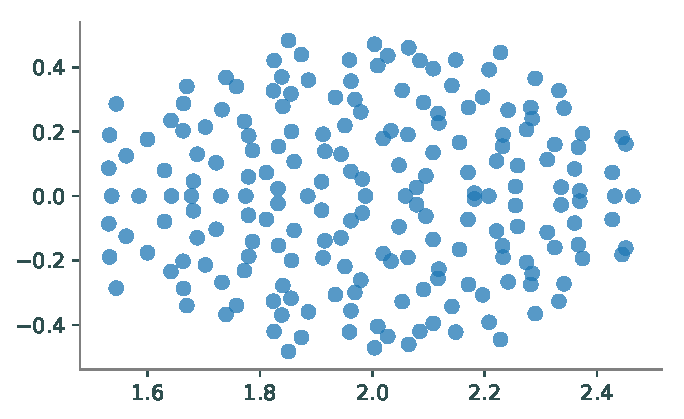
\includegraphics[width=\textwidth]{figures/scatter_gmres.pdf}
\end{subfigure}
%
\begin{subfigure}{.49\textwidth}
    \centering
    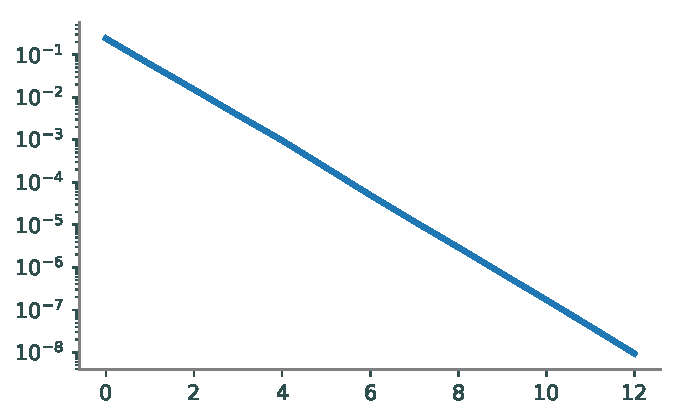
\includegraphics[width=\textwidth]{figures/gmres_convergence.pdf}
\end{subfigure}
\caption{On the left, the eigenvalues of the matrix $A_2$ defined in Problem \ref{prob:make_plots}.
On the right, the rapid convergence of the GMRES algorithm on $A_2$ with starting vector $\b = (1, 1, \ldots, 1)$.}
\label{fig:plot_gmres}
\end{figure}
\end{problem}

% This section is poorly written. It is vague, not mathematically precise.
% If we ever want to include it, then it needs a lot of work.
\begin{comment}
\subsection*{Optimizing Least-Squares for GMRES (Optional)} % -----------------

The Hessenberg structure and the Krylov subspace relations enable us to save time on the least-squares part of the problem if we use QR factorization.
Observe that if $H_n$ can be factored as $Q_n R_n$, where $Q_n$ is not the same matrix as above and $R_n$ is invertible upper triangular, we may solve the least squares problem by simply solving $R_n x_n=\norm{b} Q_{n}^{H}e_1$ via back substitution.
There are two ways in which we can speed up this process.
First, we take advantage of the Hessenberg structure by using the techniques from Problem \ref{prob:givens_hessenberg} in Lab \ref{lab:givens}.
Recall that the technique in this situation was to use Givens rotations to eliminate the subdiagonal elements one at a time.
This process, which was part of a previous lab, reduces the operation count from $O(n^3)$ to $O(n^2)$.
The second speedup comes from the fact that we already know the QR factorization for $H_{n-1}$ from the previous step of the algorithm.
This means that we can simply update the QR factorization from the previous step rather than computing it all over again.
Since $H_{n}$ has only one more column and row than $H_{n-1},$ all we need to do is update the last column by performing all previous Givens rotations on just the last column of $H_n$, which requires only $O(n)$ work.
Then we perform one final Givens rotation on $H_n$ to eliminate the new subdiagonal entry which was not present in $H_{n-1}$.
Thus, the QR factorization of $H_n$ can be reduced from an $O(n^3)$ process to only $O(n)$ using these special techniques.

The back substitution necessary to solve the least squares problem can also be reduced to an operation of $O(n)$.

The speedup from $O(n^3)$ to $O(n)$ is very good, but it can only partially alleviate the problems that come with a problem that is ill-suited for GMRES.
It may still be useful because it allows us to perform more iterations in a reasonable amount of time.
In many situations, the simple technique of the next section will keep $n$ low enough that the optimizations from this section are not critical.

 \begin{problem}
 \label{prob:GMRES2}
 (Optional) Modify MyGMRES to incorporate these optimizations, and call this program MyGMRES1.
 Run both programs on a series of five random $100\times 100$ matrices and compare the time each requires.
 Are the gains substantial?
 Try it again matrices of size $1000\times 1000$ or larger, and see how substantial the difference becomes.
 Try the same thing using the techniques of the next section.
 Explain why the difference in performance is less dramatic this time.
 \end{problem}
\end{comment}

\section*{GMRES with Restarts} % -------------------------------------------

The first few iterations of GMRES have low spatial and temporal complexity.
However, as $k$ increases, the $k$th iteration of GMRES becomes more expensive temporally and spatially.
In fact, computing the $k$th iteration of GMRES for very large $k$ can be prohibitively complex.

This issue is addressed by using GMRES(k), or GMRES with restarts.
When $k$ becomes large, this algorithm restarts GMRES with an improved initial guess.
The new initial guess is taken to be the vector that was found upon termination of the last GMRES iteration run.
\begin{comment}
GMRES with restarts is outlined in Algorithm \ref{alg:gmres_k}.

\begin{algorithm}
\begin{algorithmic}[1]
\Procedure{GMRES(k)}{$A, \b, \x_0, k, tol, restarts$}
  \State $n \gets 0$ \Comment{Initialize}
   \While{$n \leq restarts$}
	\State{ Perform the GMRES algorithm, obtaining a least squares solution $\y$}.
	\State{ If the desired tolerance was reached, return. Otherwise, continue.}
    \State $\x_0 \gets \y$
    \State $n \gets n + 1$
    \EndWhile
    \State \pseudoli{return} $\y, \,\, res$		\Comment{Return the approximate solution and the residual}
\EndProcedure
\end{algorithmic}
\caption{The GMRES(k) algorithm. This algorithm performs GMRES on a vector $\b$ and matrix $A$. It iterates $k$ times before restarting.
It terminates after $restarts$ restarts or when the residual is less than $tol$, returning an approximate solution to $A\x=\b$ and the error of this approximation. }
\label{alg:gmres_k}
\end{algorithm}
\end{comment}
The algorithm GMRES(k) will always have manageable spatial and temporal complexity, but it is less reliable than GMRES.
If the true solution $\x$ to $A\x=\b$ is nearly orthogonal to the Krylov subspaces $\mathcal{K}_n(A, \b)$ for $n\leq k$, then GMRES(k) could converge very slowly or not at all.

\begin{problem}
Write a function that implements GMRES with restarts as follows.
\begin{enumerate}
\item Perform the GMRES algorithm for a maximum of k iterations.
\item If the desired tolerance was reached, terminate the algorithm.
If not, repeat step 1 using $x_k$ from the previous GMRES algorithm as a new initial guess $x_0$.
\item Repeat step 2 until the desired tolerance has been obtained or until a given maximum number of restarts has been reached.
\end{enumerate}
Your function should accept all of the same inputs as the function you wrote in Problem 1 with the exception of $k$, which will now denote the number of iterations before restart (defaults to $5$), and an additional parameter \li{restarts} which denotes the maximum number of restarts before termination (defaults to $50$).
\label{prob:GMRESk}
\end{problem}

\section*{GMRES in SciPy} % ===================================================

The GMRES algorithm is implemented in SciPy as the function \li{scipy.sparse.linalg.gmres()}.
Here we use this function to solve $A\x=\b$ where $A$ is a random $300 \times 300$ matrix and $\b$ is a random vector.

\begin{lstlisting}
>>> import numpy as np
>>> from scipy import sparse
>>> from scipy.sparse import linalg as spla

>>> A = np.random.rand(300, 300)
>>> b = np.random(300)
>>> x, info = spla.gmres(A, b)
>>> print(info)
3000
\end{lstlisting}

The function outputs two objects: the approximate solution $\x$ and an integer \li{info} which gives information about the convergence of the algorithm.
If \li{info=0} then convergence occured; if \li{info} is positive then it equals the number of iterations performed.
In the previous case, the function performed 3000 iterations of GMRES before returning the approximate solution $\x$.
The following code verifies how close the computed value was to the exact solution.
\begin{lstlisting}
>>> la.norm((A @ x) - b)
4.744196381683801
\end{lstlisting}

A better approximation can be obtained using GMRES with restarts.
\newpage
\begin{lstlisting}
# Restart after 1000 iterations.
>>> x, info = spla.gmres(A, b, restart=1000)
>>> info
0
>>> la.norm((A @ x) - b)
1.0280404494143551e-12
\end{lstlisting}
This time, the returned approximation $\x$ is about as close to a true solution as can be expected.

\begin{problem}
Plot the runtimes of your implementations of GMRES from Problems 1 and 4 and \li{scipy.sparse.linalg.gmres()} use the default tolerance and \li{restart=1000} with different matrices.
Use the $m \times m$ matrix $P$ with $m=25,50,\dots 200$ and with entries taken from a random normal distribution with mean 0 and standard deviation $1/(2\sqrt{m})$.
Use a vector of ones for $\b$ and a vector of zeros for $\x_0$.
Use a single figure for all plots, plot the runtime on the $y$-axis and $m$ on the $x$-axis.
\end{problem}

\begin{comment}
% This problem is a potential application problem that could be included in the lab.
% The solutions to this problem are included in solutions.py.
\begin{problem}
Using the function \li{finite_difference()} from your iterative solvers lab, modify the \li{hot_plate()} function to use the GMRES algorithm instead of the SOR method.
Do you see any differences in speed?
Can you solve larger systems with GMRES?
Try the different versions of the GMRES algorithm that we have discussed, what differences do you see?
\end{problem}
\end{comment}
